\documentclass[conference]{IEEEtran}
\usepackage[utf8]{inputenc}
\usepackage[T1]{fontenc}
\usepackage[brazilian]{babel}
\usepackage{graphicx,booktabs,array,tabularx}
\usepackage{amsmath,amssymb,cite,url,etoolbox}
\usepackage{balance}
\usepackage{float}
\usepackage[hidelinks]{hyperref}
\graphicspath{{figuras/}}
\newcolumntype{Y}{>{\raggedright\arraybackslash}X}
\newcolumntype{L}[1]{>{\raggedright\arraybackslash}p{#1}}
\newcommand{\grupo}[2]{\addlinespace[1pt]\multicolumn{#1}{@{}l}{\textit{#2}}\\}
\newcommand{\inteira}[2]{\multicolumn{#1}{@{}>{\raggedright\arraybackslash}p{\columnwidth}@{}}{#2}\\}
\newcommand{\tabfont}{\fontsize{7.4}{8.8}\selectfont}
\setlength{\emergencystretch}{1em}
\renewcommand{\IEEEkeywordsname}{Palavras-chave}
\AtBeginEnvironment{thebibliography}{\renewcommand{\footnotesize}{\fontsize{7.0}{8.1}\selectfont}}
\makeatletter
\def\section{\@startsection{section}{1}{\z@}{1.7ex plus .4ex minus .2ex}{0.5ex plus .2ex}{\normalfont\normalsize\centering\scshape}}
\def\subsection{\@startsection{subsection}{2}{\z@}{1.15ex plus .3ex minus .2ex}{0.3ex plus .2ex}{\normalfont\normalsize\itshape}}
\makeatother
% Tabelas ficam exatamente onde estão no fonte ([H]), sempre entre dois parágrafos.
% \interlinepenalty impede que um parágrafo se divida entre colunas: toda coluna fecha em fim de parágrafo, e nenhuma figura ou tabela corta um parágrafo.
\interlinepenalty=10000
\AtBeginEnvironment{table}{\renewcommand{\arraystretch}{1.00}\setlength{\tabcolsep}{2pt}}
\widowpenalty=10000
\clubpenalty=10000
\displaywidowpenalty=10000
\finalhyphendemerits=10000
\setlength{\parfillskip}{0pt plus 0.86\columnwidth}
\renewcommand{\topfraction}{1}
\renewcommand{\dbltopfraction}{1}
\renewcommand{\textfraction}{0}
\setlength{\intextsep}{5pt plus 3pt minus 2pt}
\setlength{\abovecaptionskip}{1pt}
\setlength{\belowcaptionskip}{1pt}
\title{\vspace{-8pt}\fontsize{14}{16}\selectfont REV-P · Transferência de conhecimento físico por IA geoespacial auditável para análise de suscetibilidade a inundações em comunidades brasileiras com poucos registros\vspace{-12pt}}
\author{\IEEEauthorblockN{Gabriela Sofia, Bárbara Borges, Nicole Guarnieri e Rafaella Guerra}
\IEEEauthorblockA{Bacharelado em Ciência da Computação -- Pontifícia Universidade Católica do Paraná (PUCPR)\\
\{gabriela.milani, barbara.borges, nicole.guarnieri, rafaella.guerra\}@pucpr.edu.br}}
\setlength{\textfloatsep}{5pt plus 2pt minus 1pt}
\setlength{\dbltextfloatsep}{5pt plus 2pt minus 1pt}
\setlength{\floatsep}{5pt plus 2pt minus 2pt}
\setlength{\dblfloatsep}{5pt plus 2pt minus 2pt}

\IEEEaftertitletext{\vspace{-20pt}}
\hypersetup{pdftitle={REV-P: transferência de conhecimento físico por IA geoespacial auditável},pdfauthor={Gabriela Sofia, Barbara Borges, Nicole Guarnieri e Rafaella Guerra}}
\linespread{0.985}
\begin{document}
\selectfont
\maketitle
\raggedbottom
\begin{abstract}
O REV-P (Reconhecimento de Evidências Verificáveis para Predição) é uma ferramenta e um método de inteligência artificial geoespacial para analisar a suscetibilidade a cheias em comunidades com poucas observações locais. O método aprende relações entre terreno, drenagem e água em cheias documentadas e avalia sua transferência para territórios brasileiros. A ferramenta apresenta uma ordem de suscetibilidade, explica a contribuição das variáveis e identifica as fontes. Quando há imagens de radar adequadas, um módulo de visão computacional detecta água e acrescenta essa evidência à resposta.
\end{abstract}
\begin{IEEEkeywords}
Suscetibilidade a cheias; transferência; IA geoespacial; evidências verificáveis; territórios vulnerabilizados.
\end{IEEEkeywords}

%======================================================================
% INTRODUÇÃO
%======================================================================
\section{Introdução}
% A figura do método está aqui, no início do fonte, para ocupar o topo da página 2.
\begin{figure*}[!t]
\refstepcounter{section}\label{sec:metodo}\pdfbookmark[1]{Método da ferramenta}{secmetodo}
{\centering\normalfont\normalsize\scshape\Roman{section}. Método da ferramenta\par}
\vspace{2pt}
{\normalfont\normalsize\noindent A Fig.~\ref{fig:metodo} sintetiza o percurso dos dados, da observação da cheia à resposta por território.\par}
\vspace{3pt}
\centering
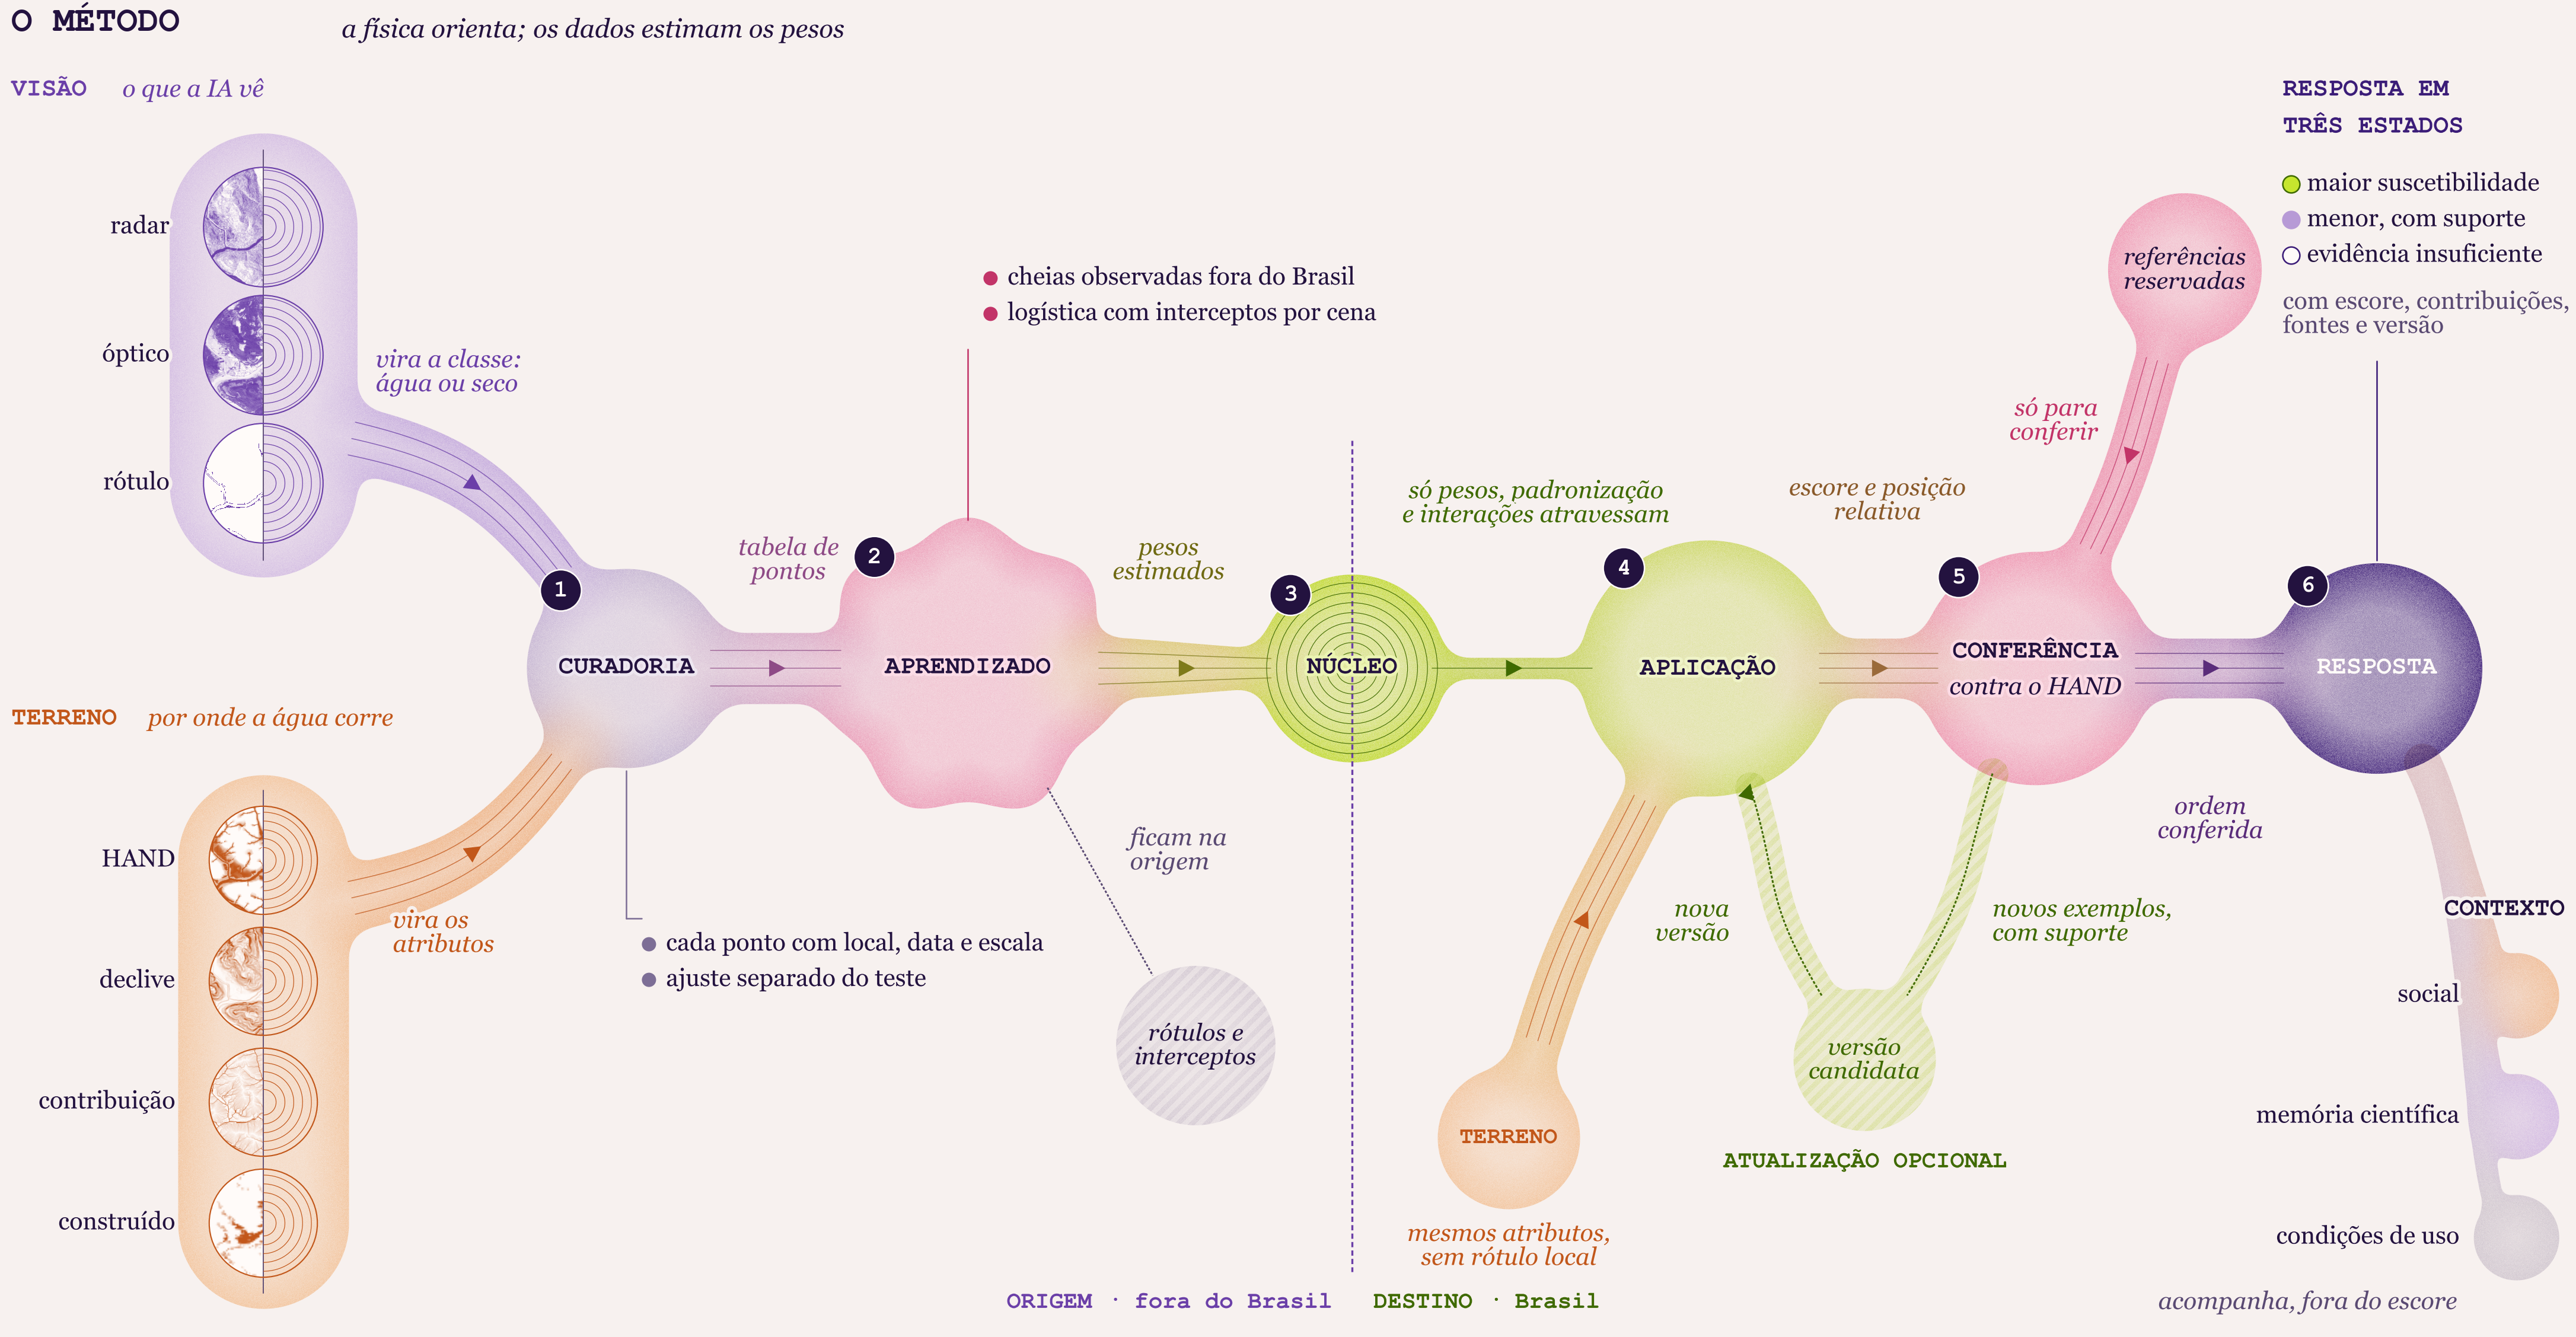
\includegraphics[width=0.88\textwidth]{fig1_metodo.png}
\caption{Fluxo do REV-P. Lilás indica as observações que geram rótulos e laranja, os atributos do terreno. Rosa marca o ajuste e a conferência com referências reservadas. Verde acompanha a transferência dos pesos e a atualização opcional. Roxo indica a resposta com escore, suporte, fontes e contexto.}
\label{fig:metodo}\end{figure*}

Uma enchente é, ao mesmo tempo, um fenômeno físico e um acontecimento na vida de alguém: a água segue o relevo, mas o que ela leva embora depende de quem mora no caminho \cite{adger}. No Brasil, o Instituto Brasileiro de Geografia e Estatística (IBGE) inclui a localização em áreas de risco ambiental entre os critérios que identificam as 12.348 Favelas e Comunidades Urbanas (FCU), onde vivem cerca de 16,4 milhões de pessoas \cite{ibge}. A observação do fenômeno nesses territórios é escassa: no acervo inicial do projeto, apenas uma comunidade tinha água observada, e nenhuma reunia locais com e sem água em número suficiente para ajuste e avaliação locais. A falta de registros reduz tanto a visibilidade das ocorrências quanto a evidência disponível para analisá-las.

Tal escassez de referências une o problema social ao desafio científico: os registros que dão visibilidade às ocorrências vividas pelas comunidades também sustentam o aprendizado e a avaliação dos modelos. Uma inteligência artificial (IA) aprende com os exemplos disponíveis, e quem nunca entrou no registro também não entra na resposta. A literatura sobre mapeamento de suscetibilidade urbana a inundações já reúne cerca de 160 abordagens \cite{islam}. Essa diversidade metodológica, contudo, não eliminou a dificuldade de levar o aprendizado a lugares distintos dos de treino, e modelos guiados só por dados podem se apoiar em correlações espúrias e super-representar as regiões mais ricas em dados \cite{bentivoglio,zhu}. Esperar que cada comunidade acumule os próprios registros seria aceitar que ela só possa ser analisada depois de inundar muitas vezes.

Este trabalho parte de outra possibilidade: como a água responde ao terreno segundo as mesmas leis em qualquer lugar, aquilo que se aprende onde o fenômeno foi bem observado pode carregar conhecimento para onde ele nunca foi. A hidrologia levou a bacias sem monitoramento um modelo treinado em 531 bacias, e a ideia alcançou a suscetibilidade urbana e o mapeamento orbital de cheias \cite{kratzertw,nearing,zhao,ratte}. Restava verificar se esse conhecimento chega às comunidades brasileiras.

A pergunta que guia o trabalho é: \textbf{como uma IA geoespacial auditável pode aprender mecanismos transferíveis de suscetibilidade urbana a enchentes, a partir de evidências físicas, observacionais, sociais e científicas, e levá-los a territórios brasileiros com pouca referência local, preservando limites de validação?}

O Reconhecimento de Evidências Verificáveis para Predição (REV-P) responde com um método e uma ferramenta. O método qualifica observações de cheia, aprende em 59 eventos no exterior como combinar atributos do terreno e aplica os pesos, sem ajuste local, para ordenar pontos em territórios brasileiros. A ordem é confrontada com evidências reservadas e pode ser atualizada com exemplos locais, enquanto unidades fora do treino medem se o aprendizado da origem se preserva.

A ferramenta apresenta, por coordenada, a posição relativa do local, a contribuição de cada variável, a versão do modelo, as fontes e o suporte da resposta, inclusive quando a evidência é insuficiente. Camadas sociais do Censo contextualizam quem vive nos lugares analisados, uma busca documental recupera a literatura, e uma etapa de verificação examina se as fontes sustentam as afirmações. A contribuição reside em articular um método que separa o que se aprende do que se verifica a uma ferramenta que torna auditável cada resposta.

A visão computacional atua em três frentes. A comparação de cenas ópticas de antes e durante a cheia e as delimitações orbitais qualificadas indicam onde houve água, fornecendo os rótulos do ajuste e as referências de conferência. Uma rede U-Net delimita a água em imagens de radar, que observam a superfície sob nuvens, e essa delimitação acompanha a resposta como evidência observacional. O treino mascarado oculta blocos do radar e do terreno e treina a rede para reconstruí-los, o que aproveita imagens sem rótulo onde as anotações são raras. O escore é calculado com o terreno e permanece disponível onde não há imagem da cheia: a imagem observa e confere, e o terreno viabiliza a transferência.

\vspace{-3pt}
Os destinos respondem a perguntas complementares. A Região Metropolitana de Porto Alegre (RMPA), em maio de 2024, reúne 6.117 dos 10.545 positivos e permite avaliar a transferência e o que poucos exemplos locais acrescentam. Manaus (Rio Negro, 2021) e a Região Metropolitana de Curitiba (RMC, Iguaçu, 2023) estendem o teste a outras bacias e episódios. Recife e sua região metropolitana (RMR) separam a capital do entorno em 2022, e, nela, os atendimentos da Defesa Civil permitem testar a ordenação por rua. Petrópolis examina outro fenômeno: as cicatrizes de deslizamento de 2022 registram rupturas de encosta, processo distinto do acúmulo de água, e conferem um modelo próprio. Em todos, o resultado é uma priorização relativa, e não uma previsão de quando ou com que profundidade a água chegará.

%======================================================================
% MÉTODO DA FERRAMENTA
%======================================================================
\subsection{Curadoria das observações}
O inventário reúne 1.641.356 observações e registra, para cada uma, local, data, fonte, escala, classe e usos autorizados. Cada observação é classificada como presença, comparador, água permanente ou evidência insuficiente, segundo o fenômeno e o instrumento. A curadoria identificou 763.155 registros aptos ao treino e 513.530 à avaliação externa, e a separação entre ajuste e teste é definida em cada ensaio.

Para o ajuste externo, agrupamos 36.331 pontos em 43 unidades de evento e sub-bacia: 16.633 de delineações do Copernicus Emergency Management Service (CEMS), 11.698 de rótulos manuais do UFO (3~m) e 8.000 do Sen1Floods11 (10~m) \cite{cems,ufo,sen1}. O teste externo usa manchas MODIS do Global Flood Database (GFD, 250~m) \cite{tellman}. Mancha é o contorno da área atingida, traçado em imagem de satélite; o GFD e o ciclone Idai a usam por cobrir regiões sem medição.

Muçum (RS) ilustra a referência óptica: cenas Sentinel-2 de 21 de abril e 6 de maio de 2024 (Fig.~\ref{fig:imagens}e--f). O índice de água por diferença normalizada modificado (MNDWI, h) compara o verde com o infravermelho de ondas curtas, faixa em que a água absorve a radiação. Marca-se água se o índice for positivo em leitura válida de 20~m \cite{xu}.

A classificação de cena (SCL), painel (m), exclui nuvem, sombra e falta de dado. Água nova exige índice positivo na cheia e leitura anterior válida sem água; um ponto válido sem água durante a cheia serve de comparador. Água anterior ou permanente, com apoio da camada do Joint Research Centre quando disponível, e leituras insuficientes ficam em classes à parte \cite{jrc}.

As manchas do CEMS de maio de 2024 (EMSR720) integraram só o núcleo congelado, avaliado fora do Brasil.

\begin{figure}[H]\centering
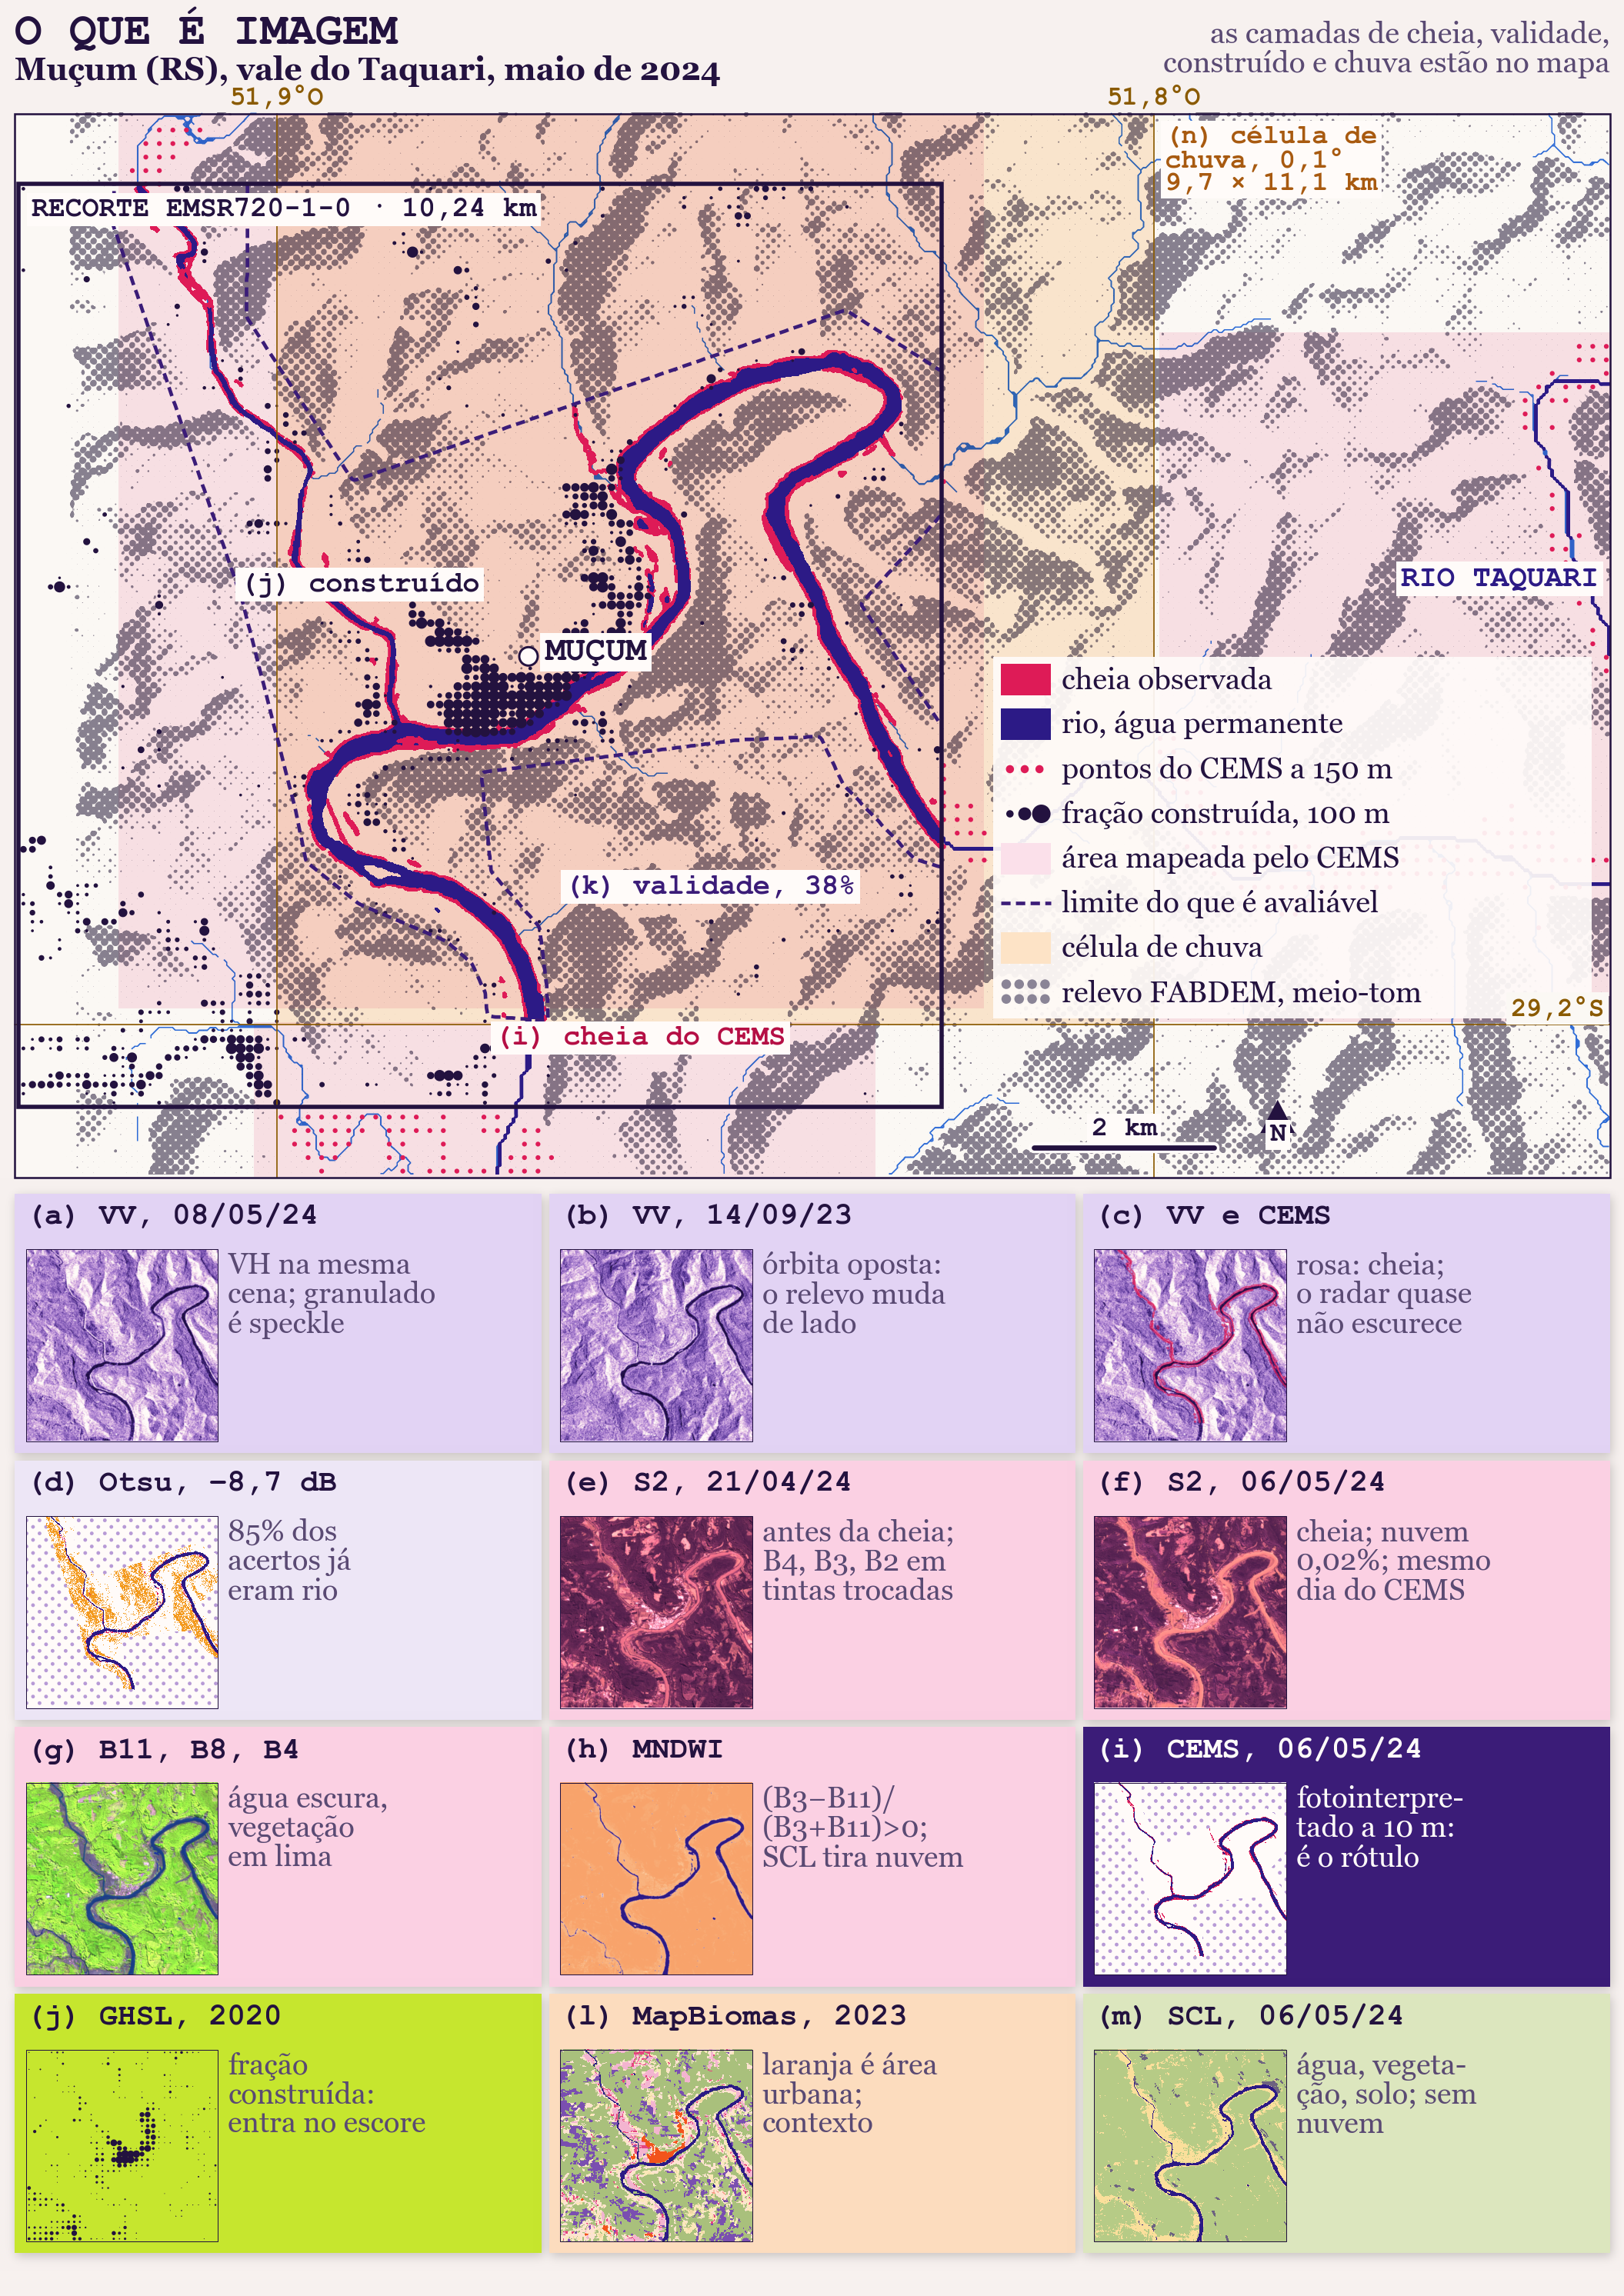
\includegraphics[width=0.94\columnwidth]{fig2_fontes_produtos.png}
\caption{Muçum (RS). Cenas antes e durante a cheia (e--f), índice de água (h), validade da leitura (m) e referência independente do CEMS (i), delimitada por analistas em imagem Pléiades Neo do mesmo dia. Recorte ilustrativo.}
\label{fig:imagens}\end{figure}

A RMPA testa a versão treinada no exterior, com a cena Sentinel-2 de 6 de maio, validada com uma mancha Planet/SkySat do Guaíba \cite{ufrgs}.

Em Recife, localizamos por endereço os relatos à Defesa Civil e reunimos os registros pela unidade rua--bairro. As ruas com relato são comparadas às demais do próprio bairro, o que reduz diferenças de notificação. Como a extensão da rua pode influenciar o registro, repetimos a análise com pares de comprimento semelhante \cite{sedec,phillips}.

Em Petrópolis, o Instituto Nacional de Pesquisas Espaciais (INPE) mapeou, pelo Charter, as cicatrizes de fevereiro de 2022, e as células fora delas formam o fundo. O inventário histórico da UFRJ/GEOCART localiza danos por endereço e amplia o registro nas comunidades \cite{inpe,geocart}.

\subsection{Atributos do terreno}
O IBGE fornece os contornos georreferenciados das FCU, que sobrepomos a um modelo digital de terreno por unidade para extrair atributos em células de cerca de 30~m, no interior e no entorno das comunidades. Assim, a ferramenta consulta o terreno por coordenada, e a análise separa os pontos das FCU dos do recorte urbano \cite{fabdem}.

Na Fig.~\ref{fig:aprendizado}, a elevação (c) informa a altitude e o declive (d) mede a inclinação local. Para calcular o \emph{Height Above Nearest Drainage} (HAND, e), seguimos o caminho de escoamento D$\infty$ até a drenagem conectada e subtraímos a cota desta da cota do ponto. A regra HAND prioriza os pontos de menor altura, que uma elevação menor do nível da água na drenagem é suficiente para alcançar \cite{hand}.

A área de contribuição (f) é o terreno a montante que drena até o ponto. As distâncias à drenagem e aos canais com contribuição $\geq$10~km$^2$ medem a conexão à rede. Com HAND, declive, fração construída (GHSL) e areia (SoilGrids), elas formam os sete atributos do núcleo, e o declive mediano do recorte modula as interações. Em Recife, os atributos são agregados por rua dentro do bairro. A chuva situa o evento no tempo e fica fora do escore \cite{beven,ghsl,soilgrids}.

\subsection{Aprendizado e transferência}
A regressão logística regularizada aprende a distinguir pontos rotulados com água dos comparadores. Cada evento recebe o mesmo peso total, com as classes balanceadas em seu interior, e um intercepto ajusta o nível do escore em cada cheia \cite{prentice}. Para o ponto \(i\), cada atributo padronizado \(x_{ij}\) contribui com seu peso \(\beta_j\). Nos pares selecionados \(\mathcal I\), o peso \(\gamma_{jk}\) multiplica o produto dos atributos, o que permite, por exemplo, que a contribuição da distância à drenagem varie com o relevo do recorte:
\[
s_i
= \sum_j \beta_j x_{ij}
+ \sum_{(j,k)\in\mathcal I} \gamma_{jk} x_{ij}x_{ik}.
\]

No destino, extraímos os mesmos atributos em cada coordenada (Fig.~\ref{fig:aprendizado}l) e aplicamos a padronização, os pesos e as interações da origem; os interceptos ficam nas cheias de ajuste.

O escore é a soma das contribuições e determina a posição relativa de cada ponto, de modo que a equação identifica os termos que separam pontos com HAND semelhante.

A versão externa completa atende à avaliação nas comunidades. A versão com reserva ajusta 29 unidades e mantém 14 fora do treino para responder ao que a completa não alcança: se os pesos dependem das unidades de ajuste e se uma atualização local preserva o que foi aprendido. Essas 14 unidades também calibram a resposta, e essa versão serve às ruas de Recife e à atualização local. Para o teste fora do país, ajustamos o núcleo congelado com 91.446 observações, incluindo eventos brasileiros.

Petrópolis requer outro modelo, pois o deslizamento decorre da ruptura da encosta, governada por inclinação e forma do terreno, enquanto a água se acumula nas partes baixas \cite{merz}. A relação também foi aprendida fora do Brasil, no inventário de 14.900 rupturas do ciclone Idai (Zimbábue, 2019), com outra regressão logística sobre sete atributos do FABDEM a 30~m e sem HAND \cite{dille}.

\begin{figure}[H]\centering
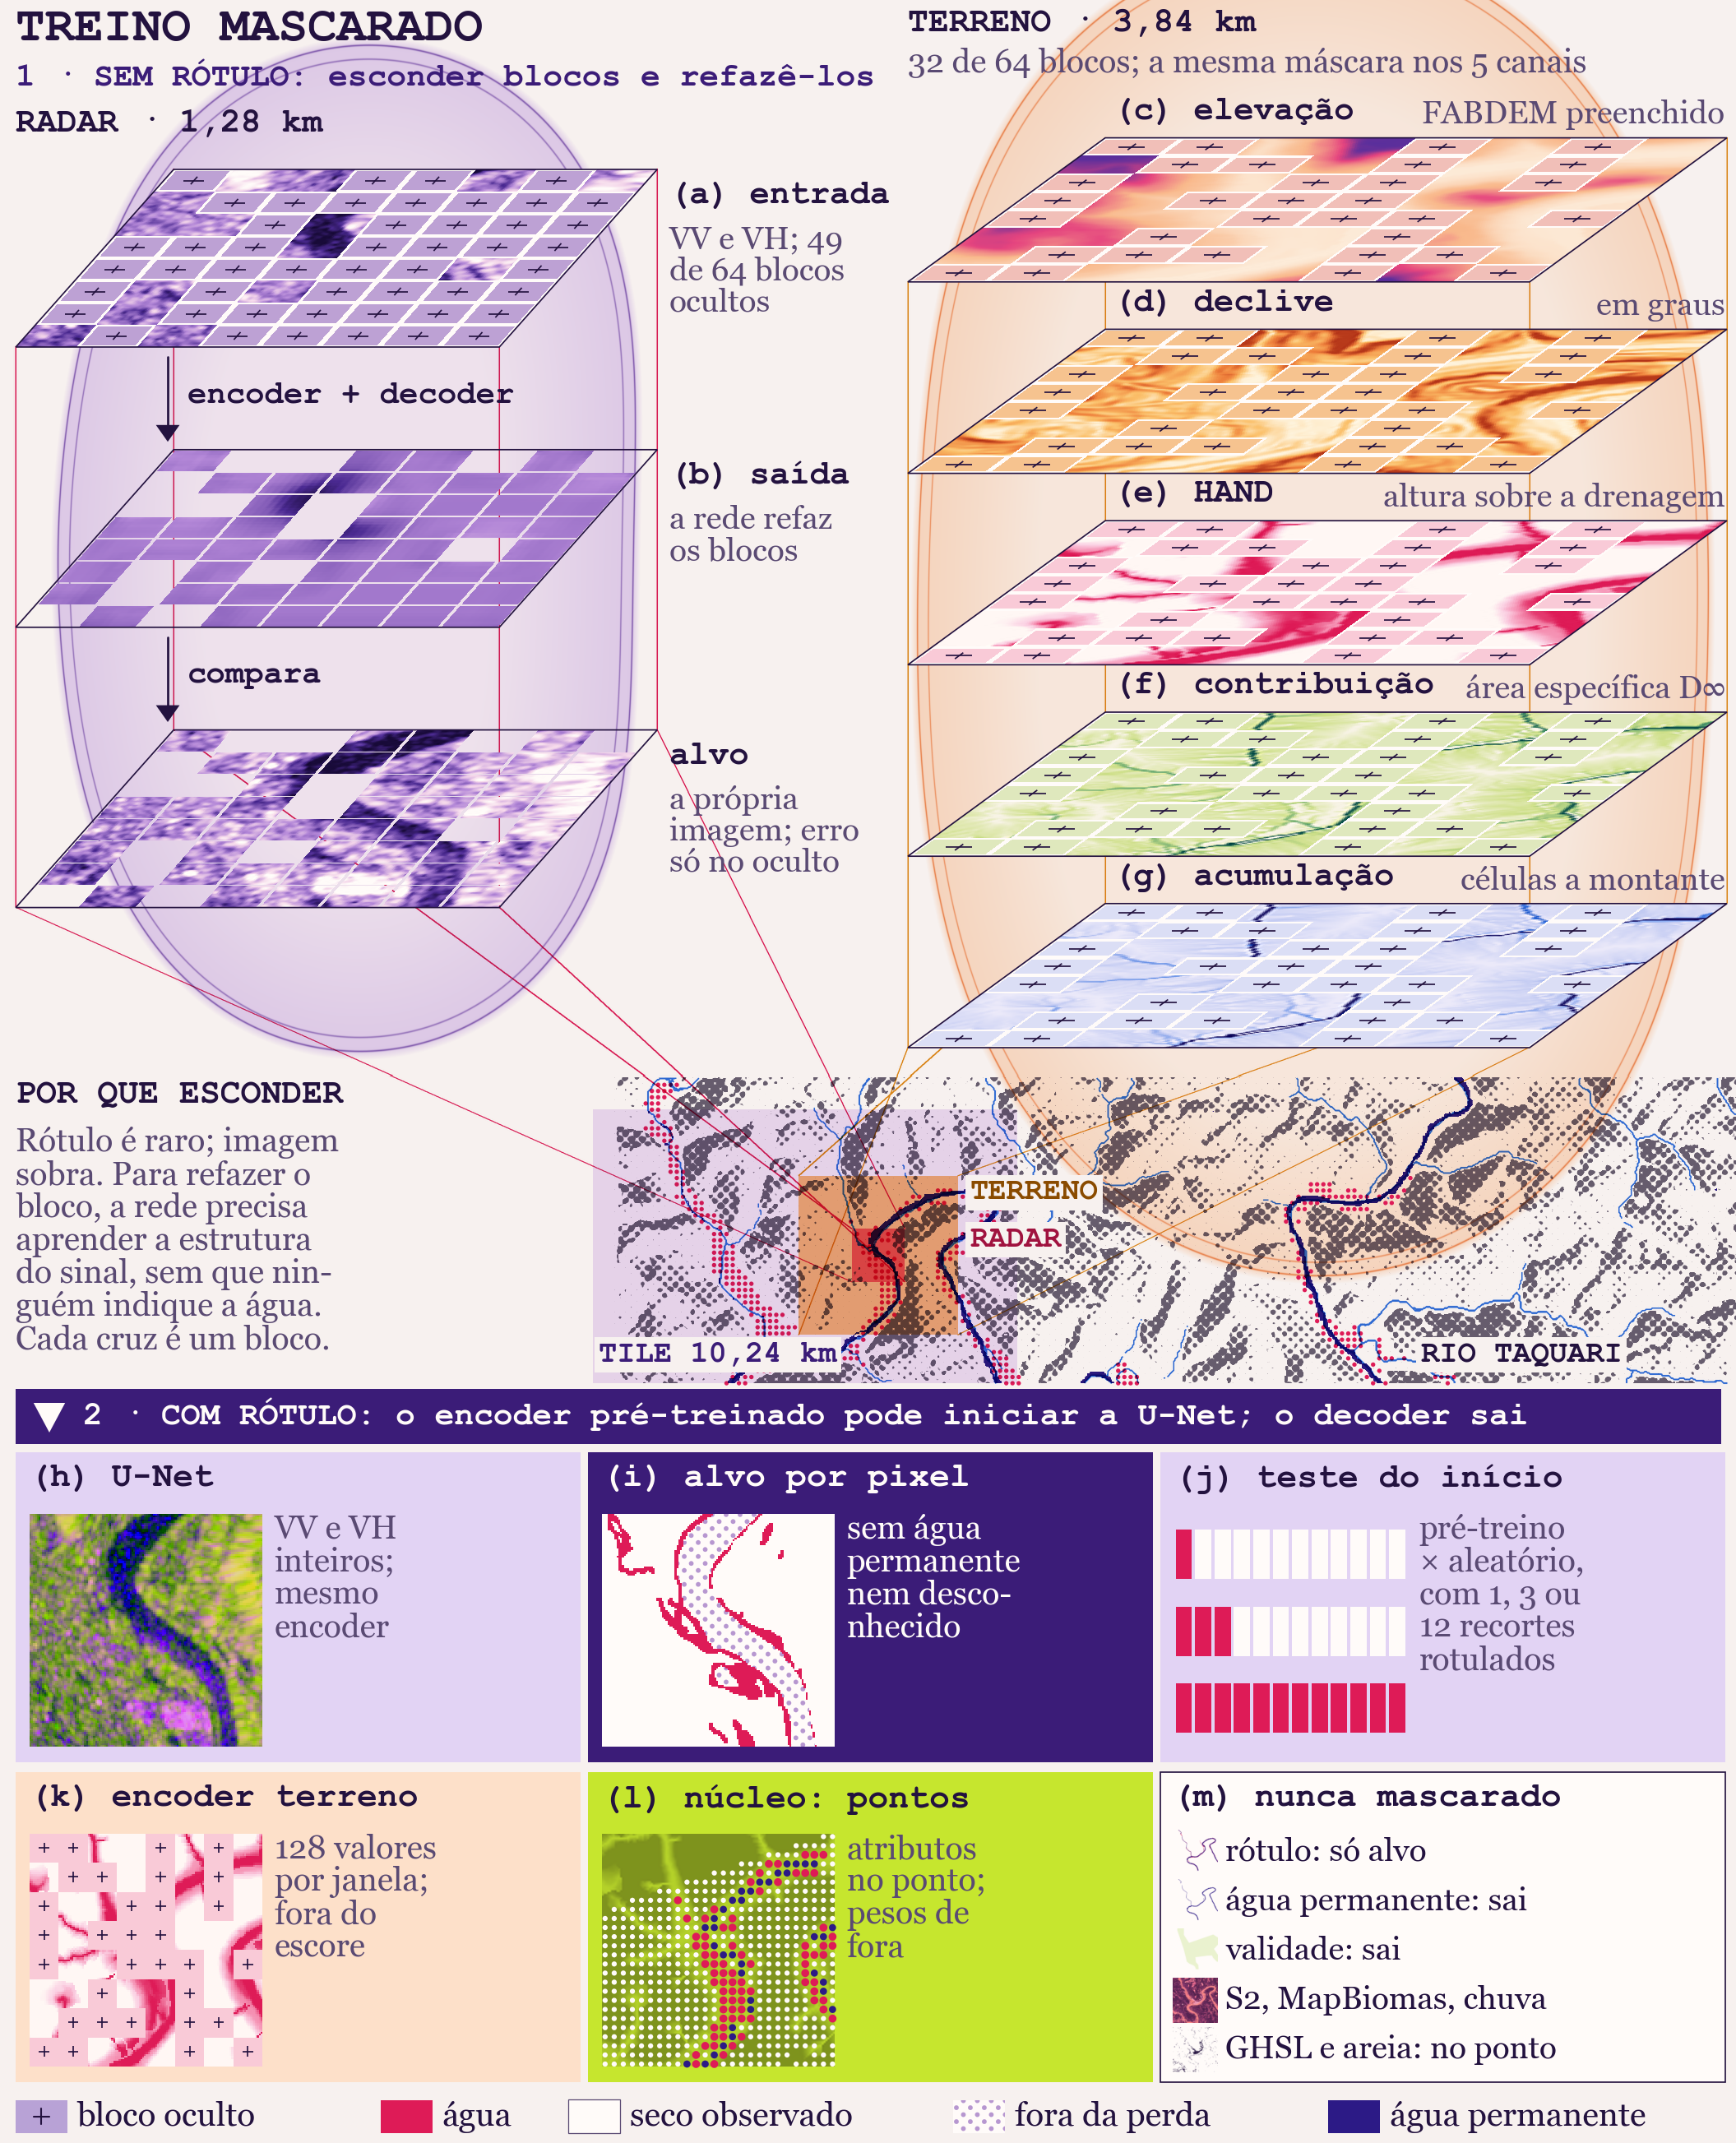
\includegraphics[width=\columnwidth]{fig_treino_mascarado.png}
\caption{Treino mascarado em Muçum (RS). Sem rótulo, a rede refaz blocos ocultos do radar (a--b) e do terreno (c--g). O encoder pode iniciar a U-Net (h--i), e o teste compara esse início ao aleatório (j). O núcleo lê atributos por ponto (l). O pré-treino usa Sen1Floods11; a saída (b) é demonstrativa.}
\label{fig:aprendizado}\end{figure}

Para identificar a água do evento, uma U-Net recebe as polarizações VV e VH do radar de abertura sintética (SAR) do Sentinel-1 e segmenta a água pixel a pixel, inclusive sob nuvens (Fig.~\ref{fig:aprendizado}h--i). Usamos 446 recortes anotados, com 90 para teste.

A interseção sobre união (IoU) divide a área comum à máscara estimada e à referência pela área coberta por ao menos uma delas \cite{unet}.

Como recortes anotados são escassos, o pré-treino mascarado aproveita imagens sem rótulo (Fig.~\ref{fig:aprendizado}a--b). A rede recebe o radar com 75\% dos blocos de 16$\times$16 pixels ocultos e reconstrói VV e VH. O erro é calculado apenas nos blocos ocultos com leitura válida, o que obriga o encoder a representar o contexto em vez de copiar a entrada \cite{mae}. O decoder é então descartado, e o encoder, idêntico ao da U-Net, pode iniciar o ajuste supervisionado.

Para medir a utilidade desse início, comparamos em oito eventos do Sen1Floods11 a rede pré-treinada à iniciada aleatoriamente, com 1, 3 ou 12 recortes rotulados por contexto (Fig.~\ref{fig:aprendizado}j). A métrica é a precisão média (AP), e uma vantagem exige intervalo acima da margem de 0,025. No terreno, o mesmo procedimento oculta metade dos blocos de cinco camadas (c--g) e produz 128 valores por janela de 3,84~km (k), mantidos fora do escore. No ajuste em sequência, o método Learning without Forgetting (LwF) usa as saídas da rede anterior para preservar o aprendizado \cite{lwf}.

\subsection{Avaliação e atualização}
\label{sec:avaliacao}
Em cada destino, o REV-P e a regra HAND ordenam os mesmos pontos, e as duas ordens são cruzadas com a referência reservada: nas coortes brasileiras, a comparação das cenas Sentinel-2 identifica água nova e comparadores (Fig.~\ref{fig:imagens}e--f); no teste externo, as manchas do GFD cumprem esse papel.

A área sob a curva ROC (AUC) resume a conferência por pares. Em cada par, formado por um ponto com água e um comparador, conta-se um acerto se o ponto com água vier primeiro e meio acerto em caso de empate. AUC de 0,80 equivale a oito acertos a cada dez pares; uma ordem ao acaso tem AUC esperada de 0,50, e uma ordem perfeita, de 1,00. Cada AUC mede a tarefa própria de sua unidade: células, ruas ou cicatrizes \cite{wadoux}.

O ganho da combinação de atributos é a AUC do REV-P menos a AUC da regra. Sua incerteza vem de 2.000 reamostragens pareadas de grupos inteiros, como comunidades nas FCU e componentes de cheias no teste externo, para não tratar pontos vizinhos como independentes.

Um intervalo todo acima de zero sustenta a vantagem do REV-P. Cada estrato avaliado reúne ao menos 20 pontos com água, distribuídos em pelo menos 10 grupos. No teste externo do núcleo congelado, hipótese, população e regra de decisão foram definidas antes da análise, com nível de confiança ajustado para três hipóteses.

A associação entre HAND e água é estimada dentro de cada cheia e entre pontos próximos, o que reduz a influência das diferenças entre eventos e regiões. A retirada de famílias de atributos mede o que cada uma acrescenta à ordenação, e a avaliação em unidades deixadas de fora, uma de cada vez, indica se o ganho sobre o HAND se repete em cheias ausentes do ajuste \cite{peters}.

A atualização incorpora exemplos do destino sem refazer o aprendizado externo. A referência é consultada em \(B\) pontos, escolhidos perto do limiar de decisão, onde o modelo mais hesita, ou por sorteio, e uma correção regularizada soma-se ao escore transferido: \(s_i^{(B)} = s_i^{(0)} + r_B(\boldsymbol x_i)\).

A correção entra em uso com ao menos cinco positivos, cinco negativos e três grupos positivos; sem esse suporte, a ferramenta conserva a versão externa. O ganho é medido no destino e a retenção, nas unidades reservadas \cite{lopezpaz}.

\subsection{Resposta e auditoria}
O mapa classifica cada local em maior suscetibilidade, menor suscetibilidade com suporte ou evidência insuficiente, e uma resposta baixa só aparece onde há base para ela. A triagem é avaliada pelos pontos com água que deixam de receber resposta baixa quando a seleção por margem substitui a aleatória, com a mesma meta de cobertura. Os dados do Censo acrescentam quem vive em cada comunidade, se houve água observada e se há ao menos cinco pontos de cada classe.

A resposta vem acompanhada do que a sustenta. A busca documental separa a literatura científica dos registros de procedência, e sua capacidade de achar a fonte certa é medida em consultas sintéticas de fonte conhecida. O exame de cada frase combina regras e um juiz que avalia se a fonte a sustenta. A auditoria numérica recompõe o escore a partir dos atributos e da versão, o que a torna reproduzível.

%======================================================================
% RESULTADOS
%======================================================================
\section{Resultados}
\subsection{Relações físicas e ganho no teste externo}
A Tabela~\ref{tab:origem} examina a relação física, mede o ganho sobre o HAND fora do ajuste e, com a reserva, mostra se os pesos dependem das cheias de treino.

\begin{table}[H]\centering
\caption{Relações aprendidas. O sinal do HAND se repete entre territórios, e a conexão à drenagem acrescenta informação no teste externo.}\label{tab:origem}\tabfont\vspace{-3pt}
\begin{tabularx}{\linewidth}{@{}Y r L{3.3cm}@{}}
\toprule
Comparação ou condição & Estimativa & IC ou referência\\\midrule
\grupo{3}{HAND e água observada}
Muçum: mediana do HAND & 2,2~m com água & 61,2~m no comparador\\
Dentro da cheia, 331.492 pontos$^{a}$ & $-$1,13 & [$-$1,31; $-$0,96]\\
Pares a até 3~km$^{a}$ & $-$1,27 & [$-$1,48; $-$1,05]\\
\inteira{3}{HAND maior, menos água em 25 de 27 territórios.}
\grupo{3}{Diferença de AUC ao testar 43 unidades, uma por vez}
Modelo geral $-$ HAND & +0,039 & [0,026; 0,054], 33 a favor\\
Retirar pistas de acumulação & $-$0,064 & [$-$0,080; $-$0,048], 39 pioram\\
\grupo{3}{Teste externo: diferença de AUC}
Núcleo $-$ HAND$^{b}$ & \textbf{+0,055} & [0,024; 0,086]\\
Com $-$ sem atributos de conexão$^{b}$ & \textbf{+0,030} & [0,006; 0,053]\\
Regressão $-$ HAND, 16 cheias$^{c}$ & \textbf{+0,041} & 13/16, $p$=0,011\\\bottomrule
\end{tabularx}
\par\vspace{2pt}
\begin{tabularx}{\linewidth}{@{}Y r r Y r r@{}}
\toprule
Peso por atributo & Completa & Reserva & Peso por atributo & Completa & Reserva\\\midrule
HAND (log) & $-$0,981 & $-$0,904 & Areia & $-$0,051 & $-$0,202\\
Distância ao canal & $-$0,429 & $-$0,433 & Contribuição (log) & +0,043 & +0,085\\
Declive & $-$0,312 & $-$0,274 & Dist. à drenagem & +0,030 & +0,055\\
Fração construída & $-$0,210 & $-$0,170 &  & & \\\bottomrule
\end{tabularx}
\par\smallskip\raggedright Pesos: versões completa e com reserva (14 unidades fora do ajuste). Os sete atributos conservam o sinal. IC95\%, exceto $^{b}$. $^{a}$Log da razão de chances por desvio-padrão de HAND. $^{b}$Núcleo ajustado com dados brasileiros e testado em 30 grupos do GFD fora do país. IC98,33\%. $^{c}$Cheias sul-americanas fora do Brasil.
\end{table}

\subsection{Transferência para comunidades brasileiras}
Os pesos aprendidos no exterior foram aplicados às comunidades e ao recorte urbano de cada destino (Tabela~\ref{tab:transferencia}). O primeiro bloco mede a tarefa que motiva o método, o segundo verifica se a vantagem se mantém na área inteira, e o último reúne duas verificações da conferência.

\begin{table}[H]\centering
\caption{Transferência sem ajuste local. Nas comunidades de Manaus, Recife e RMR, o REV-P superou o HAND.}\label{tab:transferencia}\tabfont\vspace{-3pt}
\begin{tabularx}{\linewidth}{@{}L{1.04cm}r L{2.12cm}Y r@{}}
\toprule
Nas FCU & Pos. (FCU) & AUC do REV-P & $\Delta$ HAND [IC] & $\Delta$ declive\\\midrule
RMPA & 241 (17) & 0,880 [0,828; 0,923] & --- & ---\\
Manaus & 48 (10) & 0,920 [0,791; 0,967] & \textbf{+0,046} [0,020; 0,069] & \textbf{+0,111}\\
Recife & 31 (19) & 0,866 [0,777; 0,935] & \textbf{+0,064} [0,012; 0,125] & \textbf{+0,151}\\
RMR & 366 (35) & 0,809 [0,721; 0,866] & \textbf{+0,116} [0,069; 0,145] & \textbf{+0,093}\\
\end{tabularx}
\par\vspace{2pt}
\begin{tabularx}{\linewidth}{@{}L{1.04cm}r r Y r r r@{}}
\toprule
Área & Pos. & AUC & $\Delta$ HAND [IC] & $\Delta$ declive & Baixa renda & Ref. urb.\\\midrule
RMPA & 6.117 & 0,905 & \textbf{+0,016} [0,005; 0,025] & --- & 0,884 & 0,907\\
Manaus & 215 & 0,791 & \textbf{+0,036} [0,0004; 0,061] & \textbf{+0,105} & --- & 0,804\\
RMC & 883 & 0,811 & --- & \textbf{+0,056} & --- & 0,812\\
Recife & 448 & 0,781 & \textbf{+0,043} [0,019; 0,068] & \textbf{+0,087} & 0,844 & 0,739\\
RMR & 2.882 & 0,775 & \textbf{+0,085} [0,055; 0,106] & \textbf{+0,069} & 0,770 & 0,748\\
\end{tabularx}
\par\vspace{2pt}
\begin{tabularx}{\linewidth}{@{}L{2.6cm}Y@{}}
\toprule
Rótulos embaralhados & Queda de AUC de 0,30 a 0,63\\
Outro sensor & 99\% dos positivos da RMPA na mancha Planet/SkySat\\\bottomrule
\end{tabularx}
\par\smallskip\raggedright Pos.: pontos com água nova. Entre parênteses, FCU com água. Área: recorte inteiro, com pontos fora das FCU (10.545 positivos). Baixa renda e ref. urb.: AUC por estrato. $\Delta$: AUC do REV-P menos a da regra indicada. Colchetes: IC95\%. ---: sem vantagem sustentada ou abaixo do mínimo de positivos. RMC, FCU: 11 positivos. Sentinel-2: RMPA 05/2024, Manaus 06/2021, RMC 11/2023, Recife e RMR 05/2022. RMR exclui Recife.
\end{table}

\subsection{Ordenação de ruas com relatos em Recife}
Os relatos avaliam o escore por rua, e a decomposição de duas vias do mesmo bairro mostra o que explica sua posição (Tabela~\ref{tab:relatos}).

\begin{table}[H]\centering
\caption{Recife. O REV-P priorizou ruas com relatos melhor que o HAND; a decomposição abre a conta em duas ruas de Estância.}\label{tab:relatos}\tabfont\vspace{-3pt}
\begin{tabularx}{\linewidth}{@{}Y r L{2.2cm}@{}}
\toprule
Comparação dentro do bairro & Resultado & IC ou referência\\\midrule
\inteira{3}{2014--2024: 1.648 relatos, 420 localizados até a rua, 96 ruas em 38 bairros.}
\inteira{3}{Em 16 de 71 bairros com registro, a ocorrência apareceu apenas nos relatos.}
\grupo{3}{Teste: 48 ruas com relato em 19 bairros, entre 2.225 ruas}
AUC do REV-P & 0,669 & [0,564; 0,775]\\
AUC do HAND & 0,595 & [0,491; 0,711]\\
Ganho de AUC sobre o HAND & \textbf{+0,074} & [0,012; 0,159]\\
Ruas com relato no topo de 20\% & 42\% & HAND: 31\%\\
Ganho em pares de comprimento semelhante$^a$ & +0,058 & [$-$0,024; 0,177]\\
\end{tabularx}
\par\vspace{1pt}
\begin{tabularx}{\linewidth}{@{}Y r r Y r r@{}}
\toprule
Parcela do escore & Muriti & Av. Recife & Parcela do escore & Muriti & Av. Recife\\\midrule
HAND (log) & +0,751 & +0,204 & Areia & +0,033 & +0,033\\
Dist. ao canal & +0,853 & +0,093 & Área que drena (log) & +0,129 & $-$0,013\\
Declive & +0,272 & +0,123 & Dist. à drenagem & $-$0,026 & +0,023\\
Fração construída & $-$0,525 & $-$0,406 & \textbf{Escore final} & \textbf{1,487} & \textbf{0,057}\\
\multicolumn{4}{@{}l}{Número de relatos} & 3 & 4\\
\multicolumn{4}{@{}l}{Ruas com escore menor (de 74)} & 72 & 12\\\bottomrule
\end{tabularx}
\par\smallskip\raggedright REV-P com reserva. Colchetes: IC95\%. $^{a}$Razão dos comprimentos até 1,5. Escore de ordenação: contribuições $\beta_jx_{ij}$ e interações ($|\gamma|\leq$0,027).
\end{table}

\subsection{Modelo de encostas em Petrópolis}
A relação aprendida no Idai foi conferida com as cicatrizes de 2022 e comparada ao modelo de água (Tabela~\ref{tab:encosta}).

\begin{table}[H]\centering
\caption{Petrópolis. O modelo de encostas ordenou as cicatrizes melhor que o modelo de água.}\label{tab:encosta}\tabfont\vspace{-3pt}
\begin{tabularx}{\linewidth}{@{}Y r L{2.1cm}@{}}
\toprule
Modelo ou comparação & AUC ou ganho & IC95\%\\\midrule
Modelo de água & 0,375 & [0,307; 0,445]\\
Modelo de encosta treinado no Idai & 0,660 & [0,593; 0,726]\\
Encosta $-$ modelo de água & \textbf{+0,286} & [0,170; 0,396]\\
Externo com exemplos locais $-$ só local$^{a}$ & \textbf{+0,126} & [0,070; 0,180]\\\bottomrule
\end{tabularx}
\par\vspace{2pt}\raggedright Avaliação: 81 cicatrizes e 12.170 células de fundo. Idai: AUC 0,885 em 13 blocos retidos de 10~km. Topo de 20\%: 40\% das cicatrizes. Registro interno passou de 5 para 20 das 42 FCU. 31 FCU a até 100~m. $^{a}$Ajustes com 100 consultas.
\end{table}

\subsection{Atualização local na RM de Porto Alegre}
A RMPA reúne exemplos suficientes para medir o ganho no destino, e a reserva revela o efeito na origem (Tabela~\ref{tab:atualizacao}).

\begin{table}[H]\centering
\caption{Atualização local. A margem melhorou a ordenação nas FCU da RMPA, e a reserva mede o efeito na origem.}\label{tab:atualizacao}\tabfont\vspace{-3pt}
\begin{tabularx}{\linewidth}{@{}Y r L{2.05cm} r@{}}
\toprule
Atualizado $-$ sem atualizar & Ganho em AUC & IC95\% & Rep.\\\midrule
\grupo{4}{FCU da RM de Porto Alegre, 400 consultas}
Margem (AUC de 0,874 a 0,926) & \textbf{+0,052} & [0,020; 0,101] & 6/6\\
Pontos escolhidos por sorteio & \textbf{+0,029} & [0,009; 0,062] & 6/6\\
\grupo{4}{Destino: amostra inteira da RM de Porto Alegre}
Atualização com 400 consultas & \textbf{+0,021} & [0,015; 0,026] & \\
\grupo{4}{Reserva da origem e memória}
Origem após ajuste por margem & $-$0,028 & [$-$0,056; $-$0,006] & \\
FCU, memória de 200 exemplos$^a$ & +0,017 & [0,006; 0,027] & \\\bottomrule
\end{tabularx}
\par\smallskip\raggedright 6/6: repetições do mesmo episódio. Retenção medida em seis unidades externas. Em Manaus e na RMC, o filtro conservou a versão externa por falta de positivos, evitando perda de 0,078 de AUC em Manaus. $^{a}$Ciclo com memória em três destinos.
\end{table}

\subsection{Cobertura observacional e módulos de apoio}
A ampliação do acervo levou a observação de água a mais comunidades (Tabela~\ref{tab:percepcao}).

\begin{table}[H]\centering
\caption{Cobertura observacional. O acervo ampliou a observação nas comunidades.}\label{tab:percepcao}
\tabfont\vspace{-3pt}
\begin{tabularx}{\linewidth}{@{}L{2.6cm}Y@{}}
\toprule
Recorte total$^{a}$ & 1.708 FCU, 2.776.821 moradores\\
FCU com água & De 1 no acervo inicial a 123 de 1.666 no recorte ampliado\\
Suporte nas 123 FCU & 119 com as duas classes. Em 38, há $\geq$5 pontos por classe.\\\bottomrule
\end{tabularx}
\par\vspace{0.5pt}\raggedright $^{a}$Universo censitário, inclui 42 FCU de Petrópolis.
\end{table}

O início pré-treinado elevou a detecção de água justamente onde há menos rótulos: com um único recorte rotulado por contexto, a precisão média subiu em sete de oito eventos (Tabela~\ref{tab:modulos}).

\begin{table}[H]\centering
\caption{Módulos de apoio, avaliados à parte do escore.}\label{tab:modulos}
\tabfont\vspace{-3pt}
\begin{tabularx}{\linewidth}{@{}Y L{5.8cm}@{}}
\toprule
Módulo & Métrica e comparação\\\midrule
Mapa de água, 90 recortes$^{b}$ & Sobreposição (IoU) da U-Net: 0,449\\
Pré-treino, 8 eventos$^{d}$ & Pré-treinado $-$ aleatório: $\Delta$AP +0,041 [0,014; 0,069], 7/8, com 1 recorte; +0,050 com 3\\
SAR contínuo, 8 unidades & LwF: $\Delta$IoU \textbf{+0,049} [0,029; 0,068], limiar 0,2\\
Busca, 11.238 consultas & Nas 5 primeiras: 44,35\% híbrida vs. 36,65\% lexical\\
Juiz + regras vs. regras (18) & Acerto: 0,722 vs. 0,444. Falsos positivos: 1 vs. 7\\
Água com resposta baixa$^{c}$ & Margem vs. sorteio: RMPA 0 vs. 35, RMR 25 vs. 130\\
Reprodução do escore & 147.798 pontos, erro máximo 3,56$\times$10$^{-15}$\\
Conferência do serviço & 2.747 testes (20/10), 922 fontes por hash, 5 portões\\\bottomrule
\end{tabularx}
\par\vspace{0.5pt}\raggedright $^{b}$Por pixel, sem água permanente; U-Net sem pré-treino. $^{c}$Nas FCU; meta de 70\% de cobertura na coorte. $^{d}$Intervalo não supera por inteiro a margem de 0,025.
\end{table}

\section{Discussão}
A recorrência do sinal do HAND tem explicação física. O descritor mede a altura do ponto em relação à drenagem, e a área de contribuição indica onde o escoamento converge e a saturação começa \cite{hand,beven}. Como esses conceitos descrevem o movimento da água, e não um lugar, espera-se que mantenham a direção entre regiões. A estabilidade não demonstra causa, mas justifica tratar como mecanismo transferível uma relação preditiva de motivação física \cite{peters}.

A transferência alcança os pesos, e não o nível do escore, pois amostrar por classe altera o intercepto da regressão logística e preserva as inclinações \cite{prentice}.

O resultado dialoga com a hidrologia de grandes amostras, em que um modelo sem dados da bacia alcançou eficiência mediana de 0,69, contra 0,64 do modelo calibrado em cada uma das 531 bacias \cite{kratzertw}. O alvo ali é a vazão no tempo, e as métricas não se comparam, mas o princípio é o mesmo. A transferência em suscetibilidade urbana já contornou a escassez de inventários em bacias de Pequim, e o mapeamento orbital passou a examinar a generalização fora da área de treino \cite{zhao,ratte}. O REV-P leva essa pergunta para dentro das comunidades, e sete atributos de significado físico, legíveis na resposta, bastaram para superar o HAND numa literatura com modelos de 5 a mais de 20 parâmetros \cite{islam}.

O significado social está na observação. A exposição das favelas já foi medida em escala global \cite{lislum}. Aqui se acrescenta a conferência dentro delas, onde a vantagem sobre o HAND foi maior do que na área inteira em Manaus, Recife e na RMR. Como a ausência de chamado não equivale à ausência de água, comparar ruas dentro do bairro aplica o princípio de que o fundo deve partilhar o viés de registro das presenças \cite{phillips}.

A fronteira do que se transfere é dada pelo processo. Cheias de origens físicas distintas pedem leituras distintas \cite{merz}. Em Petrópolis, o modelo de água ficou abaixo do acaso nas cicatrizes, e o aprendido nas rupturas do Idai as ordenou, pois a água procura as partes baixas, e a ruptura nasce na encosta \cite{dille}.

Conhecimento externo e observação local se somam. O ganho maior das consultas por margem é o esperado quando a informação nova se concentra na fronteira de decisão, e medir separadamente ganho e retenção faz da reserva um critério de uso \cite{lopezpaz}. Na percepção, o início pré-treinado é útil justamente com poucos rótulos, finalidade do treino mascarado \cite{mae}.

Como AUC por grupos não equivale à acurácia de um mapa, a ferramenta apresenta a ordenação como priorização relativa \cite{wadoux}. Os ensaios nas coortes brasileiras são de desenvolvimento, e confirmar a transferência em comunidades inéditas pede episódios independentes.

\section{Conclusão}
Em resposta à pergunta de pesquisa, uma IA geoespacial auditável pode aprender relações físicas em cheias documentadas e transferi-las, sem ajuste local, aos territórios brasileiros avaliados: a direção da relação se repete, a combinação de atributos superou a regra HAND no teste externo e em Manaus, Recife e na RMR, e cada resposta expõe sua conta, suas fontes e o que falta observar. Quando o processo muda, como nas encostas de Petrópolis, o método aprende outro modelo com a mesma lógica, e, onde há exemplos suficientes, a atualização local soma-se ao que veio de fora.

O projeto entrega um método que separa o que se aprende do que se verifica e uma ferramenta que, por coordenada, devolve a ordem de suscetibilidade, a contribuição das variáveis, as fontes e o suporte. Para as comunidades que o motivaram, isso muda o ponto de partida: no domínio avaliado, um lugar que nunca entrou em um registro não precisa esperar pela próxima cheia para receber uma resposta fundamentada no terreno. Código e artefatos: \url{https://github.com/gabriela-sofia/flood_Audit-Service}.

\begin{thebibliography}{99}
\bibitem{adger} W. N. Adger, “Vulnerability,” \emph{Global Environ. Change}, vol. 16, pp. 268--281, 2006.
\bibitem{ibge} IBGE, \emph{Censo Demográfico 2022: Favelas e Comunidades Urbanas, resultados do universo}, 2a ed. Rio de Janeiro, 2025.
\bibitem{islam} T. Islam et al., “A systematic review of urban flood susceptibility mapping: remote sensing, machine learning, and other modeling approaches,” \emph{Remote Sens.}, vol. 17, art. 524, 2025.
\bibitem{bentivoglio} R. Bentivoglio et al., “Deep learning methods for flood mapping: a review of existing applications and future research directions,” \emph{Hydrol. Earth Syst. Sci.}, vol. 26, pp. 4345--4378, 2022.
\bibitem{zhu} X. X. Zhu et al., “On the foundations of Earth foundation models,” \emph{Commun. Earth Environ.}, vol. 7, art. 103, 2026.
\bibitem{kratzertw} F. Kratzert et al., “Toward improved predictions in ungauged basins: exploiting the power of machine learning,” \emph{Water Resour. Res.}, vol. 55, pp. 11344--11354, 2019.
\bibitem{nearing} G. Nearing et al., “Global prediction of extreme floods in ungauged watersheds,” \emph{Nature}, vol. 627, pp. 559--563, 2024.
\bibitem{zhao} G. Zhao et al., “Improving urban flood susceptibility mapping using transfer learning,” \emph{J. Hydrol.}, vol. 602, art. 126777, 2021.
\bibitem{ratte} C. Ratté-Fortin et al., “A transferable deep learning framework for flood mapping: spatial generalization across hydro-climatic regimes using satellite imagery,” \emph{Int. J. Appl. Earth Obs. Geoinf.}, vol. 149, art. 105321, 2026.
\bibitem{cems} Copernicus Emergency Management Service, \emph{Rapid Mapping: activations}, Comissão Europeia. \url{https://mapping.emergency.copernicus.eu/}
\bibitem{ufo} R. Mukherjee et al., “Urban Flood Observations: a hand-labeled training and validation dataset of post-flood inundation,” arXiv:2604.23066, 2026.
\bibitem{sen1} D. Bonafilia et al., “Sen1Floods11: a georeferenced dataset to train and test deep learning flood algorithms for Sentinel-1,” in \emph{Proc. CVPR Workshops}, 2020, pp. 835--845.
\bibitem{tellman} B. Tellman et al., “Satellite imaging reveals increased proportion of population exposed to floods,” \emph{Nature}, vol. 596, pp. 80--86, 2021.
\bibitem{xu} H. Xu, “Modification of normalised difference water index (NDWI) to enhance open water features in remotely sensed imagery,” \emph{Int. J. Remote Sens.}, vol. 27, pp. 3025--3033, 2006.
\bibitem{jrc} J.-F. Pekel et al., “High-resolution mapping of global surface water and its long-term changes,” \emph{Nature}, vol. 540, pp. 418--422, 2016.
\bibitem{ufrgs} I. Possantti et al., “Banco de dados das cheias na Região Hidrográfica do Lago Guaíba em maio de 2024,” Zenodo, 2025, doi:10.5281/zenodo.14617475.
\bibitem{sedec} SEDEC Recife, \emph{Registro de atendimentos da Defesa Civil}, dados abertos. \url{https://dados.recife.pe.gov.br}
\bibitem{phillips} S. J. Phillips et al., “Sample selection bias and presence-only distribution models: implications for background and pseudo-absence data,” \emph{Ecol. Appl.}, vol. 19, pp. 181--197, 2009.
\bibitem{inpe} INPE e International Charter Space and Major Disasters, \emph{Call 0864, Brazil RJ: componentes vetoriais de Petrópolis}, 2022. \url{https://data.inpe.br/charter}
\bibitem{geocart} UFRJ/GEOCART, \emph{Inventário histórico de deslizamentos}, camada do SIG municipal de Petrópolis. \url{https://sig.petropolis.rj.gov.br}
\bibitem{fabdem} L. Hawker et al., “A 30 m global map of elevation with forests and buildings removed,” \emph{Environ. Res. Lett.}, vol. 17, art. 024016, 2022.
\bibitem{hand} C. D. Rennó et al., “HAND, a new terrain descriptor using SRTM-DEM,” \emph{Remote Sens. Environ.}, vol. 112, pp. 3469--3481, 2008.
\bibitem{beven} K. J. Beven e M. J. Kirkby, “A physically based, variable contributing area model of basin hydrology,” \emph{Hydrol. Sci. Bull.}, vol. 24, pp. 43--69, 1979.
\bibitem{ghsl} M. Pesaresi, “GHS-BUILT-S R2023A: GHS built-up surface grid,” Comissão Europeia, JRC, 2023.
\bibitem{soilgrids} L. Poggio et al., “SoilGrids 2.0: producing soil information for the globe with quantified spatial uncertainty,” \emph{SOIL}, vol. 7, pp. 217--240, 2021.
\bibitem{prentice} R. L. Prentice e R. Pyke, “Logistic disease incidence models and case-control studies,” \emph{Biometrika}, vol. 66, pp. 403--411, 1979.
\bibitem{merz} R. Merz e G. Blöschl, “A process typology of regional floods,” \emph{Water Resour. Res.}, vol. 39, no. 12, 2003.
\bibitem{dille} A. Dille et al., “Capturing the complete landslide--debris-rich flood continuum for accurate inventory, susceptibility and exposure mapping -- lessons from Cyclone Idai,” \emph{Nat. Hazards Earth Syst. Sci.}, vol. 26, pp. 2561--2577, 2026.
\bibitem{unet} O. Ronneberger et al., “U-Net: convolutional networks for biomedical image segmentation,” in \emph{Proc. MICCAI}, 2015, pp. 234--241.
\bibitem{mae} K. He et al., “Masked autoencoders are scalable vision learners,” in \emph{Proc. CVPR}, 2022, pp. 16000--16009.
\bibitem{lwf} Z. Li e D. Hoiem, “Learning without forgetting,” \emph{IEEE Trans. Pattern Anal. Mach. Intell.}, vol. 40, pp. 2935--2947, 2018.
\bibitem{wadoux} A. M. J.-C. Wadoux et al., “Spatial cross-validation is not the right way to evaluate map accuracy,” \emph{Ecol. Model.}, vol. 457, art. 109692, 2021.
\bibitem{peters} J. Peters et al., “Causal inference by using invariant prediction: identification and confidence intervals,” \emph{J. R. Stat. Soc. B}, vol. 78, pp. 947--1012, 2016.
\bibitem{lopezpaz} D. Lopez-Paz e M. Ranzato, “Gradient episodic memory for continual learning,” in \emph{Proc. NeurIPS}, 2017.
\bibitem{lislum} D. Li et al., “Disproportionate flood exposure for slum populations of the Global South,” \emph{Nat. Cities}, vol. 2, pp. 626--638, 2025.

\end{thebibliography}
\end{document}
